\chapter{DebugWire}\label{chap:dw}
\section{Descrizione del protocollo e fondamentali}

Parte fondamentale del core AVR, omessa dal diagramma in \cref{fig:avr-arch}, è il sistema di \textit{debugging} on chip ``\textit{DebugWire}''.

Esso permette, tramite un tool esterno collegato all'integrato, di interrompere l'esecuzione della cpu e successivamente di effettuare operazioni di lettura e scrittura sulle memorie e sui registri.\cite[sec 25]{avr:m328p}

Affinché le funzionalità di debugging siano disponibili, è necessario abilitare la periferica DebugWire tramite i bit di configurazione al momento della programmazione del dispositivo\cite[tab 28-7]{avr:m328p}.

\subsection{Interfaccia fisica}\label{ss:dw-phy}

L'interfacciamento fisico tra controllore e dispositivo esterno avviene tramite una sola connessione al pin di reset dell'integrato \textit{target}.

Il fatto che l'interfaccia di debug sia collocata sul pin di reset comporta che, una volta abilitata la periferica DebugWire, non sia più possibile resettare il dispositivo o programmarlo tramite interfaccia ISP\cites{avr:appnote:isp}[sec 25.3]{avr:m328p}, ma si rende necessaria una procedura di disattivazione temporanea o la possibilità di programmare l'integrato tramite il protocollo DebugWire.

La comunicazione tra programmatore e target è di tipo seriale e half duplex data la natura della connessione. In particolare il protocollo utilizzato è una derivazione di una seriale UART su un bus open collector, come è osservabile dalla \cref{fig:dw-schematic}\cite{site:dw-reverse-engeneering}.

\begin{figure}[t]
    \centering
    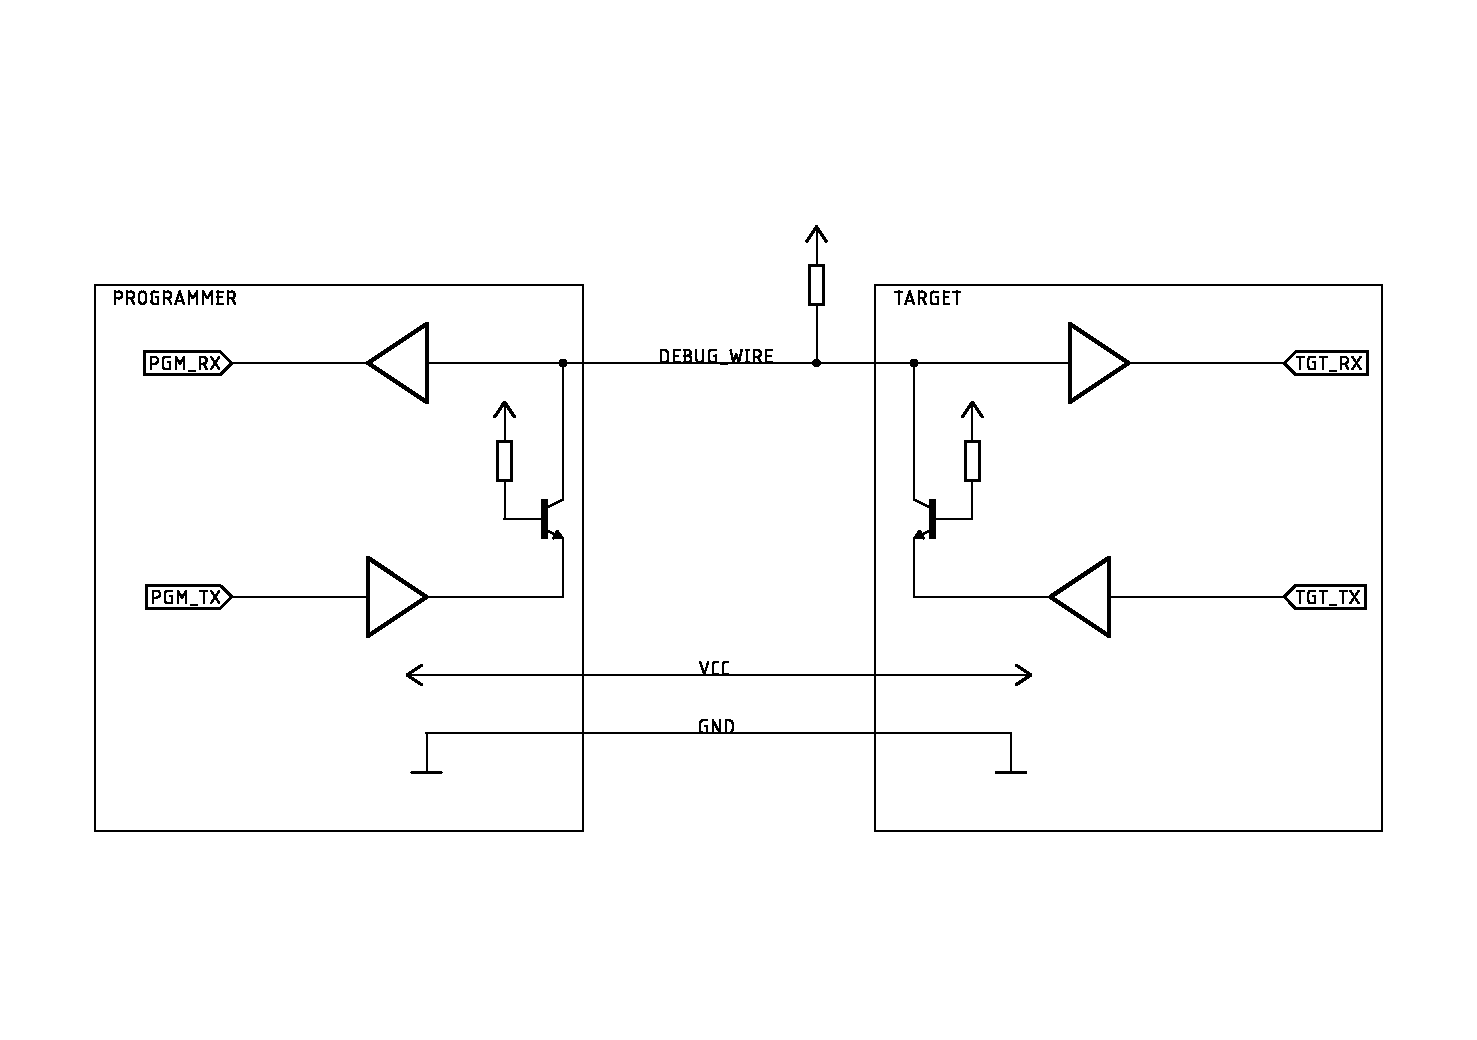
\includegraphics[width=\textwidth]{dw-schematic.pdf}
    \caption[]{Schema concettuale del funzionamento dell'interconnessione tra programmatore e controllore target per il protocollo DebugWire}\label{fig:dw-schematic}
\end{figure}

\subsubsection{Protocollo UART}\label{ss:uart}

Il protocollo UART è un metodo di trasmissione punto-punto digitale seriale asincrono che generalmente lavora su due connessioni tra i due attori della comunicazione. Le due linee rimangono a livello logico 1 quando non c'è attività.

Le linee prendono il nome di ``TX'' e ``RX'' in funzione dell'utilizzo che la periferica master ne fa: è necessario notare come le due linee vengano ``incrociate'' in modo tale da far sì che il pin di trasmissione di un attore vada a collegarsi con il pin di ricezione della controparte.

Essendo un protocollo asincrono, ovvero vi è assenza di una linea di sincronizzazione (clock), le due parti della comunicazione devono conoscere a priori la velocità e il formato dei dati attesi sulle linee.

La trasmissione inizia con un periodo di livello logico 0 (\textit{Start Bit}), in modo che sia possibile l'identificazione dell'inizio della trasmissione di un simbolo rilevando il fronte di transizione da livello logico 1 a livello logico 0 (\textit{Falling Edge}).

Durante questo tempo di bit dove la linea di trasmissione è a livello logico 0 è dunque possibile inizializzare l'hardware e sincronizzare le sorgenti di clock per la ricezione. In seguito al bit di inizio si susseguono i bit del dato, dal meno significativo al più significativo, con periodo pari al tempo di bit stesso. In funzione della specifica del protocollo possono essere inviate unità di dati fondamentali di dimensione da 5 a 8 bit.

A seguito dei bit di dati viene quindi inviato opzionalmente un bit di parità per garantire l'integrità dei dati e successivamente la linea viene posta a livello logico 1 per uno o due periodi di bit, permettendo al ricevitore di eseguire operazioni e resettare la macchina a stati per la ricezione dell'eventuale simbolo seguente.\cite{site:rs-uart}

Essendo un sistema asincrono è opportuno ipotizzare il disallineamento delle frequenze di invio e campionamento: in tal caso una desincronizzazione può essere tollerata se entro il limite dato dall'\cref{eq:uart-max-delay}
\begin{equation}\label{eq:uart-max-delay}
    t_{delay_{\max}} = \frac{1}{2}(N_{data}+N_{parity}+N_{stop}+1)t_{bit}    
\end{equation}
dove \(N_{data}\) è il numero di bit contenuti nel simbolo inviato che è stato negoziato, \(N_{parity}\) indica il numero di bit di parità, \(N_{stop}\) il numero di \textit{stop bits} e \(t_{bit}\) è il tempo per bit. Inoltre si tiene conto del bit di inizio (\textit{start bit}). Questo comportamento può essere notato dalla \cref{fig:uart-sync}, dove vengono rappresentati il caso ideale e il caso di desincronizzazione massima. In ogni caso si ha che il campionamento avviene all'interno del bit in invio.

\afterpage{
    \begin{figure}[ht]
        \centering
        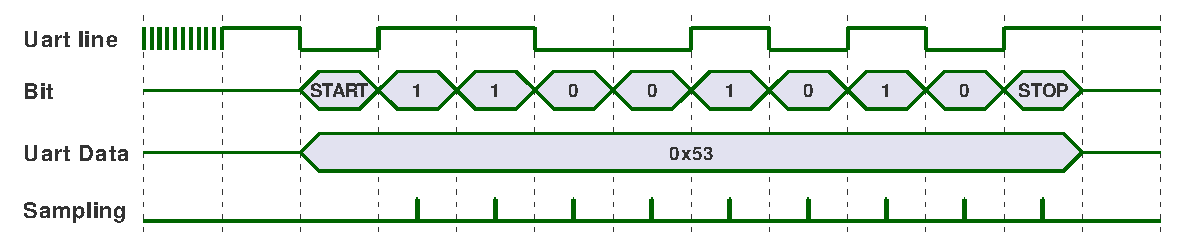
\includegraphics[width=.8\textwidth]{uart-timings.pdf}\\
        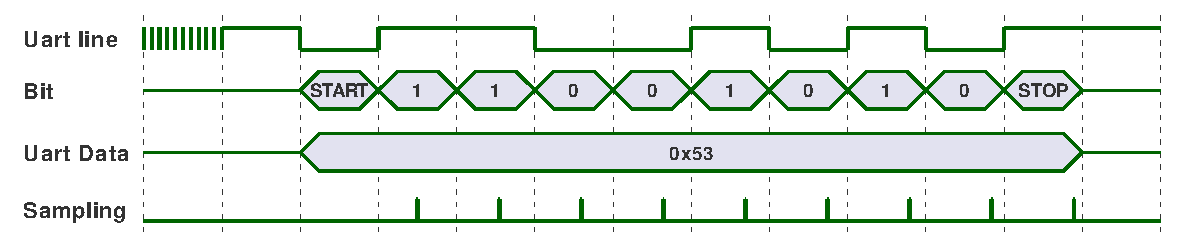
\includegraphics[width=.8\textwidth]{uart-timings-unsync.pdf}
        \caption[]{I diagrammi di sequenza dimostrano che, anche in caso di non sincronizzazione delle frequenze di invio e ricezione viene mantenuta l'integrità dei dati trasmessi. Viene mostrata una comunicazione seriale 8N1\footnote{Definizione della configurazione di una linea seriale. Essa è composta da tre caratteri: <Numero di bit dati><Tipo di parità ([N]one, [O]dd, [E]ven, [M]ark, [S]pace)><Numero di Stop bits>}}\label{fig:uart-sync}
    \end{figure}
}

La motivazione per cui il campionamento avviene a metà del tempo di bit è data dal fatto che la desincronizzazione può essere causata da una frequenza più alta o più bassa, per cui vale la relazione descritta dall'\cref{eq:uart-period-receive-delay}
\begin{equation}\label{eq:uart-period-receive-delay}
     t_{bit_{recv}} = t_{bit_{snd}} \pm t_{delay_{\max}}
\end{equation}

Infine, se la velocità di trasmissione fosse misurata in \textit{bit per secondo}, secondo la formula \(v_{uart} = \frac{1}{t_{bit}}\), essa non sarebbe veritiera e porterebbe confusione, in quanto la formula sopra enunciata includa nel conteggio dei bit trasmessi anche i bit di controllo (Start, parity e Stop bit) i quali non contribuiscono all'informazione inviata. Di conseguenza è opportuno definire la velocità di trasmissione della linea seriale come il numero di simboli trasmessi per secondo. Questa definizione differisce dalla prima un quanto il simbolo è composto da un numero di bit non necessariamente pari a 8.

È possibile determinare la velocità in baud a partire dal bitrate e dalla configurazione della linea UART secondo la relazione~\ref{eq:baud-from-bit-rate}\cite{site:baud}:
\begin{equation}\label{eq:baud-from-bit-rate}
    v_{tx_{baud}} = \frac{1}{t_{bit}(N_{data} + N_{parity} + N_{stop} + 1)}
\end{equation}

Da quanto è possibile dedurre dall'\cref{eq:baud-from-bit-rate}, l'effettivo bit rate di trasmissione della linea UART differisca di un fattore di \(\frac{N_{data}}{N_{data} + N_{parity} + N_{stop} + 1}\) rispetto al bitrate grezzo di trasmissione \(v_{uart}\)


\subsection{Funzionamento}\label{sec:dwworkings}

Tutte le comunicazioni che avvengono sul bus DebugWire non hanno alcun tipo di verifica dell'integrità del dato (Serial 8N1). La comunicazione può avvenire in qualsiasi momento.

In particolare il reset della comunicazione tra target e programmatore/debugger avviene mediante l'invio di un BREAK\footnote{La linea viene posta a livello logico 0 per più di 9 tempi di bit} sulla linea.
Ogni qualvolta sia rilevato un errore (per esempio viene ricevuto un byte inatteso o un comando non noto), il primo attore che rileva l'errore invierà un BREAK che causerà il reset della controparte.

Ciò è possibile perché la connessione è un bus open collector: il conflitto di accesso avviene solo ponendo la linea a livello logico 0 e non comporta cortocircuitazioni di qualsiasi genere. Il conflitto viene rilevato quando un attore legge dal bus uno stato diverso da quanto inviato durante la trasmissione del bit (in particolare quando l'attore riceve un bit pari a 0 quando sta inviando un bit di valore 1). Successivamente al rilevamento di un conflitto, la comunicazione viene reinizializzata allo stato originale ponendo rimedio ai conflitti di accesso. 

Il protocollo instaura una connessione a ``\textit{response -- reply if necessary}'', permettendo così di stabilire il diritto di accesso al bus in funzione dello scambio di dati precedentemente avvenuto. Se un dispositivo accede al bus quando non era suo diritto, il secondo attore effettua la procedura sopra indicata per segnalare tale violazione e reinizializzare la comunicazione.

La velocità di comunicazione è invece definita in funzione della frequenza della cpu del target. Nell'hardware della periferica è presente un \textit{prescaler} (il cui valore di default è di 128) e la velocità di comunicazione viene stabilita come \[v_{com} = \frac{f_{cpu} [Hz]}{prescaler}[bps]\]

Ad ogni reset della comunicazione il prescaler viene resettato al valore iniziale.

In risposta ad un BREAK il target risponderà sempre con l'invio di un valore noto (0x55), facendo sì che a livello fisico sia inviata un'onda quadra con frequenza \(v_{com}\)\cite{site:dw-reverse-engeneering} (si veda \cref{fig:dw-timings})

\begin{figure}[ht]
    \centering
    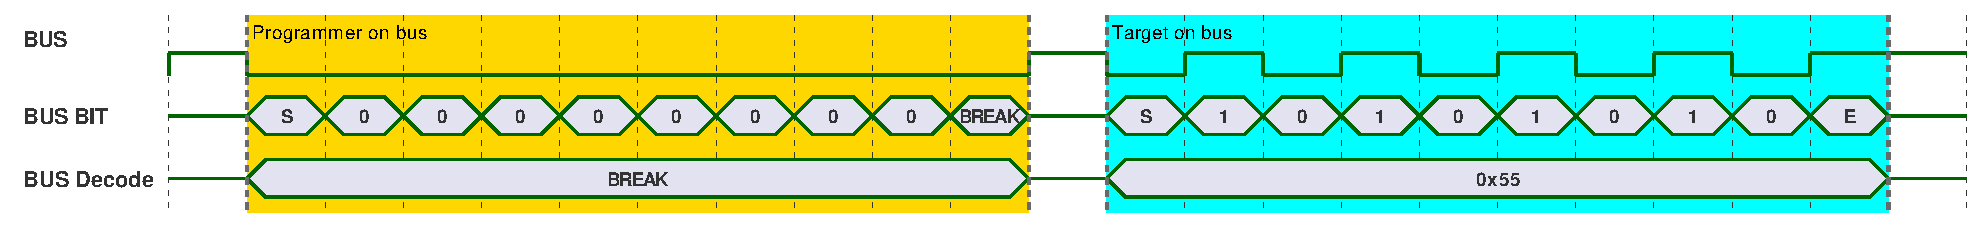
\includegraphics[width=\textwidth]{dw-break.pdf}
    \caption[]{Diagramma delle tempistiche del bus DebugWire durante il reset della trasmissione}\label{fig:dw-timings}
\end{figure}

È dunque possibile definire un algoritmo per l'inizializzazione della sessione in modo che la frequenza della trasmissione venga dedotta dalla risposta del target invece che essere nota a priori, permettendo un untilizzo semplificato della periferica.

L'algoritmo è strutturato come segue
\begin{enumerate}
    \item Preparazione dell'hardware e inizializzazione strutture dati
    \item Invio di un break dalla durata di 100ms. La durata viene stabilita in funzione della frequenza di trasmissione ragionevolmente più bassa possibile: Considerando che la famiglia AVR integra nei suoi controllori un oscillatore RC a 128kHz usato comunemente per operazioni ``low power'' e ipotizzando che sia abilitata la funzionalità di divisione del clock per un fattore di 8\cite[sec 9.11, tab 28-9]{avr:m328p}, si ottiene una frequenza del core di 16kHz. Ponendo quindi il prescaler di comunicazione DebugWire a 128 otteniamo una frequenza di trasmissione di 125Hz, ovvero 8ms per bit. Infine, sapendo che il tempo di break consiste in almeno 10 bit trasmessi a 0, si ottiene un tempo minimo di break di 80ms, arrotondato a 100ms
    \item Attesa del primo fronte di transizione da livello logico 1 a livello logico 0
    \item Attesa del successivo fronte di transizione da livello logico 0 a livello logico 1 (calcolando il tempo intercorso tra i due fronti)
\end{enumerate}

A questo punto è possibile trovare la frequenza di bit dalla quale ricavare il baud rate.

\subsection{Comandi e features}

Una volta che la cpu del controllore target è in stato \textit{halt} è possibile interagire con la periferica DebugWire per eseguire le operazioni di debug. A seguito di un BREAK e successiva risposta è possibile interpellare il controllore con i comandi descritti di seguito.

Vi sono due classi di comandi: comandi basilari e comandi composti.
I primi sono comandi che svolgono azioni semplici e definite staticamente, quali la scrittura del Program Counter, Instruction register, scrittura del registro di breakpoint hardware e configurazione di flag e comunicazione. Tramite questi comandi è possibile definire i limiti di scrittura/lettura delle memorie e eseguire istruzioni.
I Secondi sono operazioni complesse che necessitano parametri di configurazione i quali sono impostati tramite comandi basilari.

I comandi disponibili per l'interazione con il microcontrollore target tramite DebugWire sono limitati e appartengono a quattro categorie: \textit{Communication Settings}, \textit{Flag Setting},\textit{Program Flow Control} e \textit{Memory R/W}.

\subsubsection{Communication Settings}

Questi comandi vengono utilizzati per modificare il valore del prescaler di comunicazione in modo da variare la velocità di trasmissione. Sono comandi particolarmente utili nel debugging di controllori a bassa frequenza (128kHz).

Non vi è una logica nota nell'assegnazione del comando al corrispondente valore del prescaler: si rende necessaria una tabella di associazione come riportato dalla \cref{tab:dw-presc-settings}

\begin{table}[ht]
    \centering
    \begin{tabular}{ c c c }
        \textbf{Comando} & \textbf{Valore del prescaler} & \textbf{Bitrate a 16MHz} \\
        \hline
        0x83 & 128 & 125kbps \\
        0x82 & 64 & 254kbps \\
        0x81 & 32 & 500kbps \\
        0x80 & 16 & 1Mbps \\
        0xA0 & 8 & 2Mbps \\
        0xA1 & 4 & 4Mbps \\
        0xA2 & 2 & 8Mbps \\
        0xA3 & 1 & 16Mbps \\
        \hline
    \end{tabular}
    \caption[]{Tabella descrittiva dei comandi per la modifica del prescaler di trasmissione della periferica di debug del controllore target\cite{site:dw-reverse-engeneering}}\label{tab:dw-presc-settings}
\end{table}

Una volta inviato il comando di configurazione del prescaler il controllore si adatterà alla velocità richiesta e risponderà con il valore \texttt{0x55} inviato alla nuova frequenza. Questo valore può essere usato per settare adattivamente la frequenza del programmatore oppure per verificare che le impostazioni siano corrette.

\subsubsection{Flag Setting}

È necessario configurare lo stato della periferica prima di eseguire effettivamente le operazioni che sono state preparate. Possiamo chiamare questo stato ``Contesto di esecuzione'' in quanto la stessa configurazione dell'hardware permette di eseguire diverse azioni in funzione del contesto che viene configurato.

I contesti disponibili sono elencati nella \cref{tab:dw-contexts}.

\begin{table}[ht]
    \centering
    \begin{tabular}{ c l }
        \textbf{Comando dW} & \textbf{Contesto} \\
        \hline
        0x60 & Ripresa dell'esecuzione\\
        0x61 & Ripresa dell'esecuzione fino all'indirizzo HWBP\\
        0x64 & Lettura/Scrittura memoria Flash\\
        0x66 & Lettura/Scrittura della SRAM\\
        0x79 & Riprese dell'esecuzione usando l'istruzione caricata\\
        0x7A & Single Step\\
        \hline
    \end{tabular}
    \caption[]{Tabella descrittiva dei contesti di esecuzione DebugWire\cite{site:dw-reverse-engeneering}}\label{tab:dw-contexts}
\end{table}

È possibile inoltre modificare i contesti ponendo il valore del bit 5 a zero per permettere alle periferiche di temporizzazione (timers) di continuare il conteggio durante lo stepping.

\subsubsection{Program Flow Control}

Questi comandi sono utilizzati per confermare le operazioni da eseguire.

Esistono comandi di ``GO'' per le varie operazioni composite quali la lettura e scrittura della memoria SRAM (0x20 per indirizzi multipli, 0x21 per un indirizzo singolo), esecuzione di un'istruzione precedentemente caricata in IR senza incrementare il program counter (0x23), ripresa dell'esecuzione (0x30) o single stepping (0x31).

Se il bit 5 è settato allora il target effettuerà il reset della sessione inviando un BREAK seguito da 0x55 al termine dell'esecuzione.

\subsubsection{Memory R/W}\label{sss:dw-mem-io}

Questi sono i comandi fondamentali per la scrittura e lettura dei registri PC, IR, HWBP e SIGNATURE (sola lettura).

Questi registri possono essere trattati opportunamente a seconda della loro funzione oppure possono essere visti come parametri di configurazione per le operazioni composite descritte in seguito.

I registri di configurazione sono mappati da un indice come descritto dalla tabella\ref{tab:dw-regs-idx}.

\begin{table}[ht]
    \centering
    \begin{tabular}{ c l }
        \textbf{Indice} & \textbf{Registro associato} \\
        \hline
        0 & Program Counter (PC)\\
        1 & Hardware Breakpoint (HWBP)\\
        2 & Instruction Register IR\\
        3 & DW Signature register\\
        \hline
    \end{tabular}
    \caption[]{Tabella descrittiva dell'associazione degli indici ai registri elementari\cite{site:dw-reverse-engeneering}}\label{tab:dw-regs-idx}
\end{table}

Le operazioni di lettura e scrittura dei registri avvengono mediante l'invio di pacchetti come definito dalle \cref{fig:dw-reg-wrt,fig:dw-reg-rd}

\begin{figure}[ht]

    \centering
    \begin{bytefield}[endianness=big,bitwidth=1em]{24}
        \bitheader{0-23}\\
        \bitbox{4}{0xD} & \bitbox{4}{idx} & \bitbox{16}{data}\\
    \end{bytefield}

    \caption[]{Pacchetto di scrittura di un registro elementare. Nessuna risposta da parte del target}\label{fig:dw-reg-wrt}
\end{figure}


\begin{figure}[ht]

    \centering

    \begin{lrbox}{\bytefieldbox}
        \begin{bytefield}[endianness=big,bitwidth=1em]{8}
            \bitheader{0-7}\\
            \bitbox{4}{0xF} & \bitbox{4}{idx} \\
        \end{bytefield}
    \end{lrbox}
    \subfloat[]{\usebox{\bytefieldbox}}

    \vspace*{5mm}%
    \begin{lrbox}{\bytefieldbox}
        \begin{bytefield}[endianness=big,bitwidth=1em]{16}
            \bitheader{0-15}\\
            \bitbox{16}{data}\\
        \end{bytefield}
    \end{lrbox}
    \subfloat[]{\usebox{\bytefieldbox}}


    \caption[]{Pacchetto di lettura di un registro elementare (a) e successiva risposta (b)}\label{fig:dw-reg-rd}
\end{figure}

\subsubsection{Comandi compositi}

DebugWire permette di leggere e scrivere la memoria SRAM mediante una combinazione di comandi elementari.
Grazie a questa funzionalità è possibile leggere e scrivere sia la memoria dati che i registri di configurazione delle periferiche e i registri ``general purpose'' come viene evidenziato dalla \cref{fig:avr-sram-alloc}.

L'algoritmo per la scrittura dei registri (r0-r31) consiste in quanto segue\cite{site:dw-reverse-engeneering}:
\begin{enumerate}
    \item Context: SRAM R/W
    \item Scrittura del registro iniziale nel registro PC
    \item Scrittura del registro finale nel registro HWBP
    \item Selezione modalità (Comando C2 seguito dall'indice dell'operazione come descritto nella \cref{tab:dw-ops})
    \item GO SRAM R/W
    \item (Se scrittura) Invio dei byte da scrivere.\\(Se lettura) Ricezione dei byte letti.
\end{enumerate}

\begin{table}[t]
    \centering
    \begin{tabular}{ c l }
        \textbf{Indice} & \textbf{Modalità} \\
        \hline
        0 & Lettura memoria SRAM\\
        1 & Lettura registri \\
        2 & Lettura memoria Flash\\
        4 & Scrittura memoria SRAM\\
        5 & Scrittura registri\\
        \hline
    \end{tabular}
    \caption[]{Tabella descrittiva dell'associazione degli indici alle modalità di operazione sulle memorie\cite{site:dw-reverse-engeneering}}\label{tab:dw-ops}
\end{table}

Di seguito, alla \cref{fig:dw-reg-rw-com}, viene riportata la traccia di comunicazione per questo algoritmo.

Analogamente è possibile leggere e scrivere la memoria SRAM e leggere la memoria FLASH con il seguente algoritmo:
\begin{enumerate}
    \item Scrittura dell'indirizzo di partenza nella coppia di registri \texttt{r30 - r31}
    \item Scrittura del registro PC al valore 0x0000 se lettura o 0x0001 se scrittura
    \item Scrittura del doppio della lunghezza dei dati (+1 se in scrittura) da leggere/scrivere registro HWBP
    \item Selezione modalità
    \item GO con appropriata modalità.
\end{enumerate}

\begin{figure}[p]

    \centering
    \begin{bytefield}[endianness=big,bitwidth=1em]{32}
        \bitheader{0-31}\\
        \bitbox{8}{CNTX\_SRAM} & \bitbox{8}{0xD0} & \bitbox{16}{start\_reg} \\
        \bitbox{8}{0xD1} & \bitbox{16}{end\_reg + 1} & \bitbox{8}{0xC2} \\
        \bitbox{8}{MOD: 0x00/0x05} & \bitbox{8}{GO MEM}
    \end{bytefield}

    \caption[]{Comunicazione inviata dal debugger per leggere/scrivere i registri. In caso di scrittura viene seguita da (end\_reg - start\_reg) byte, altrimenti la stessa quantità di byte viene ricevuta.}\label{fig:dw-reg-rw-com}
\end{figure}

\begin{figure}[p]

    \centering
    \begin{bytefield}[endianness=big,bitwidth=1em]{32}
        \bitheader{0-31}\\
        \bitbox{8}{CNTX\_SRAM} & \bitbox{24}{0xD0001E} \\
        \bitbox{24}{0xD10020} & \bitbox{8}{0xC2} \\
        \bitbox{8}{0x05} & \bitbox{8}{0x20} & \bitbox{16}{addr\_start} \\
        \bitbox{8}{0xC2} & \bitbox{8}{0x04/0x00/0x01} & \bitbox{16}{0xD000} \\
        \bitbox{8}{0x00/0x01} & \bitbox{8}{0xD1} & \bitbox{16}{len * 2 (+1 if wrt)}\\
        \bitbox{8}{GO MEM}
    \end{bytefield}

    \caption[]{Comunicazione inviata dal debugger per leggere/scrivere le memorie. In caso di scrittura viene seguita da \textit{len} byte, altrimenti la stessa quantità di byte viene ricevuta.}\label{fig:dw-mem-rw-com}
\end{figure}

Alla \cref{fig:dw-mem-rw-com}, viene riportata la traccia di comunicazione per questo algoritmo.

È possibile eseguire direttamente un'istruzione senza scriverla nella memoria Flash. In questo caso è sufficiente scrivere nel registro IR l'opcode dell'operazione ed eseguire il comando di flow control (0x23 o 0x33). Si noti che non è possibile eseguire istruzioni di 32 bit.

Si noti come i valori dei registri \texttt{Z, PC, HWBP e IR} vengano modificati da queste operazioni. Ciò rende necessaria una procedura di salvataggio e ripristino prima di riprendere l'eventuale esecuzione del codice sul dispositivo \textit{target}.